\documentclass{article}
\usepackage{amsmath}
\usepackage{amssymb}
\usepackage{graphicx}
\usepackage{hyperref}
\usepackage[version=4]{mhchem}

\title{Problem 2}
\date{}

\begin{document}
\maketitle

\section*{Problem}
A circle is inscribed in triangle \(A B C\). The tangent points are \(D, E, F\) as shown. Show that \(\angle F D E=90^{\circ}-\frac{1}{2} \angle A\).\\
\centering
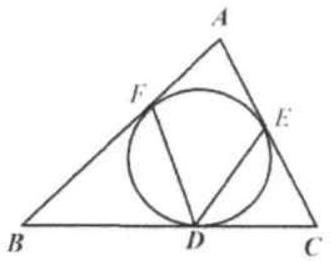
\includegraphics[width=\textwidth]{images/206(3).jpg}

\section*{Solution}
Solution not available.

\end{document}
